\documentclass{article}
\usepackage{graphicx} % for figures
\usepackage{float}
\usepackage[export]{adjustbox}
\usepackage{fancyhdr}
\begin{document}

\title{Physics 240 - Project report 2\\
		Roche surfaces}
\author{Tin Tran}

\maketitle

\section{Introduction}
This week I'm hitting a road block for my project. Initially, I planned on plotting the contour of of a simple binary star system with mass M$_1$ and M$_2$ for some random position a and b. I set up the correct equation but I could not get the correct contour plot. Below is what I got:

\begin{figure}[H]
\centering{
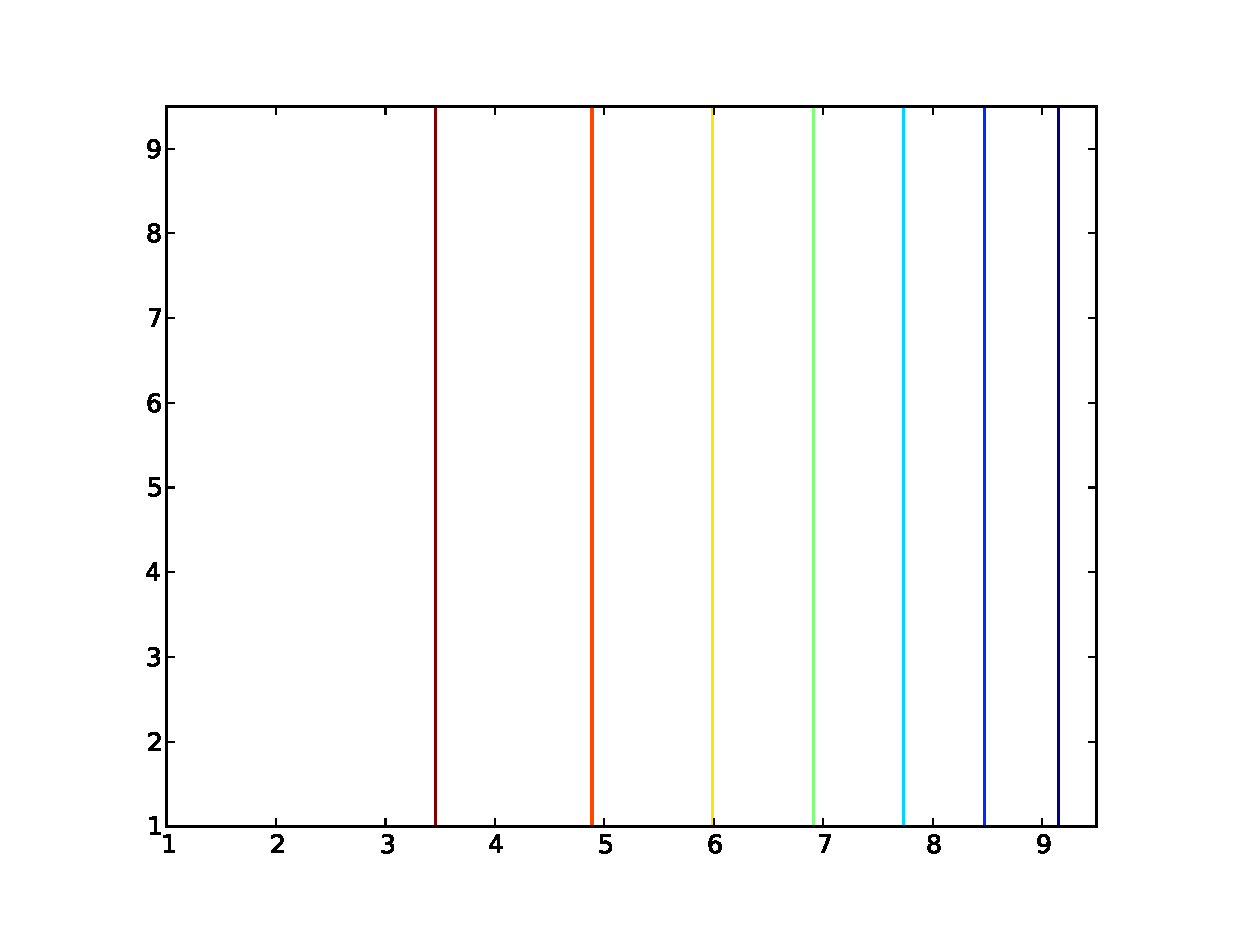
\includegraphics[max size={\textwidth}{\textheight}]{contour1.eps}
\caption{Linear fit of Global Temperature vs time}
}
\end{figure}
I have no idea why the plot looks like that. Perhaps I need to find the Lagragian points by taking the gradient of the potential, then use that for the plot. I have some question regarding this that I need to ask you.
\end{document}